\documentclass[letterpaper, 12pt]{article}
\usepackage{geometry}
\geometry{
    letterpaper,
    left=20mm,
    top=20mm,
    bottom=20mm
}
\usepackage{tocloft}
\usepackage{graphicx}
\usepackage{authblk}
\usepackage{amssymb}
\usepackage{lipsum}
\usepackage{float}
\usepackage{times}
\usepackage{amsmath}
\usepackage[format=plain,
            labelfont={bf,it},
            textfont=it]{caption}
\captionsetup{justification=raggedright,singlelinecheck=false}
\usepackage{ragged2e}
\usepackage{longtable}
\usepackage{comment}
\usepackage{setspace}
\usepackage{fancyhdr}
\usepackage{titlesec}
\usepackage[hyperindex,breaklinks]{hyperref}
\hypersetup{
    colorlinks=true,
    linkcolor=blue,
    filecolor=magenta,      
    urlcolor=blue
}
\usepackage[T1]{fontenc}
\usepackage{helvet}
\renewcommand{\familydefault}{\sfdefault}
\pagenumbering{gobble}
\usepackage[skip=10pt plus1pt, indent=40pt]{parskip}
\usepackage{orcidlink}
\usepackage{standalone}

\titlespacing*{\section}
{0pt}{1.5ex plus 1ex minus .2ex}{1.3ex plus .2ex}

\renewcommand\Authfont{\fontsize{12}{14.4}\selectfont}
\renewcommand\Affilfont{\fontsize{9}{10.8}\itshape}

\newcommand{\cosigpart}[1]{
  \addcontentsline{toc}{part}{#1}
}
\newcommand{\cosigsection}[1]{
  \section*{#1}
  \phantomsection % avoid warnings from hyperref about the anchor of a bookmark and its parent's
  \addcontentsline{toc}{section}{#1}
}
\begin{document}
\flushleft
\includegraphics[width=0.5\textwidth]{img/home/241017_final_logo_mockup.png}

\cosigpart{Biology and medicine}
\cosigsection{Antibody validation}
\textit{Last updated: 14 May 2025}

Antibodies are a very common and exceptionally useful reagent in biomedical studies. Antibodies are designed to bind to a specific kind of protein, allowing scientists to isolate that protein on a gel, tag that protein with a fluorescent probe, etc.

Antibodies are typically purchased from large laboratory supply vendors. Ideally, antibodies should be selective (i.e., they bind strongly to the protein of interest) and specific (i.e., they only bind strongly to one protein of interest). However, commercially-available antibodies can be plagued by a variety of issues:

\begin{itemize}
    \setlength\itemsep{-0.5em}
    \item \textbf{Lack of specificity:} An antibody could bind non-specifically to a number of other proteins aside from its target protein.
    \item \textbf{Lack of selectivity:} An antibody could fail to bind strongly to its target protein.
    \item \textbf{Variability in quality:} Different batches of antibody manufactured by the same provider may not perform as well as others.
    \item \textbf{Specificity to conformation:} It is possible that an antibody binds a protein only in its folded state or its unfolded state. Depending on the application, researchers may prefer an antibody that is selective and specific to one of these conformations. Even if an antibody does not bind selectively or specifically to a protein in its folded state, it may bind to the protein in its unfolded state and may still be suitable for use in application where the protein is expected to be unfolded (or vice versa).
    \item \textbf{Specificity to isoform:} The same protein can exist as a variety of \href{https://en.wikipedia.org/wiki/Protein_isoform}{isoforms}. An antibody may more effectively target one of a protein's isoforms over another.
\end{itemize}

Several initiatives have been launched to improve the quality of antibodies and the reproducibility of studies using them:

\begin{itemize}
    \setlength\itemsep{-0.5em}
    \item \textbf{\href{https://www.antibodypedia.com/}{Antibodypedia}} is an online platform that documents the level of support thousands of commercially-available antibodies have for various applications.
    \item \textbf{\href{https://www.antibodyregistry.org}{The Antibody Registry}} is an online platform that allows users to catalog the antibodies that they use in their research with rich metadata and provenance tracking (useful if an antibody is no longer sold by a vendor).
    \item \textbf{\href{https://www.citeab.com}{CiteAb}} is a service that tracks the uses of specific reagents, including antibodies, in the biomedical literature.
    \item \textbf{\href{https://www.proteinatlas.org/about/antibody+validation}{The Human Protein Atlas}} provides antibody validation data for antibodies that the project produces internally and collects validation data from suppliers for antibodies that are commercially available. 
    \item \textbf{\href{https://pabmabs.com/}{pAbmAbs}} allows users to rate antibodies out of five stars for their overall performance and for different applications.
    \item \textbf{\href{https://www.labome.com/index.html}{The Validated Antibody Database}} curates articles using and validating antibodies and collects reviews of antibodies used for a number of popular protein targets.
    \item \textbf{\href{https://ycharos.com/}{YCharos (Antibody Characterization through Open Science)}} is a non-profit that performs systematic validation of commercially-available antibodies, making their results openly available online.
\end{itemize}

This guide covers several common applications for antibodies and how they are validated for these applications according to the \href{https://doi.org/10.1038/s41596-024-01095-8}{protocol developed by YCharOS}. 

YCharOS tests antibodies in wild-type (WT) cell lines expressing the protein of interest and in knockout (KO) cell lines in which the protein of interest is `knocked out' by removing the gene encoding that protein from the cell line's genome with \href{https://en.wikipedia.org/wiki/CRISPR_gene_editing}{CRISPR-Cas9} technology.

\pagebreak

\subsection*{Western blotting/immunoblotting}

A Western blot usually involves separating proteins from cells (either from cell media for secreted proteins or from cell lysate for proteins expected to be internal to cells), separating proteins in this media/extract by running them on an \href{https://en.wikipedia.org/wiki/SDS-PAGE.}{SDS-PAGE} gel. This denatures the protein (although other varieties of gel, such as \href{https://www.med.unc.edu/pharm/sondeklab/wp-content/uploads/sites/868/2018/10/Native-gel-analysis.pdf}{native PAGE}, preserve the conformation of the protein in its native, folded state). After this, the contents of the gel are transferred to a membrane. A primary antibody that binds to the protein of interest is added to the membrane, followed by a secondary antibody that binds to the primary antibody and makes it detectable.

YCharos \href{https://f1000research.com/gateways/ycharos/faqs}{states}:

\begin{quote}
    \textit{A successful antibody immunodetects the target protein, and the signal observed in the wild-type (WT) lysate is lost in the knockout (KO) lysates. Ideally, the antibody also does not recognize any other protein under the conditions tested.}
\end{quote}

\begin{figure}[h!tbp]
    \centering
    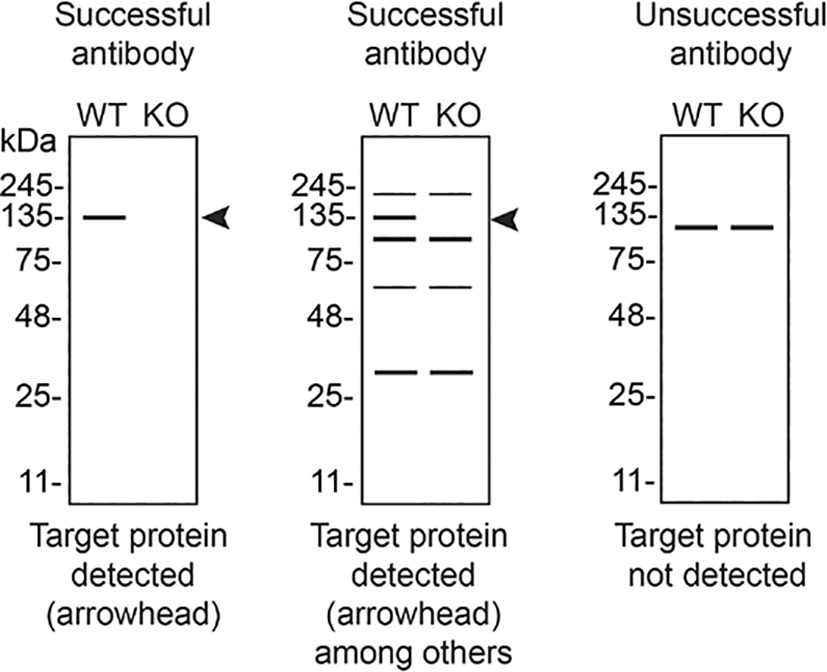
\includegraphics[width=0.9\textwidth]{img/antibody_val/ycharos_wb.jpg}
    \caption*{Schematic illustrating expected outcomes for a successful antibody (left), for a successful antibody that non-specifically binds the protein of interest (center) and a non-successful antibody (right). Adapted from Table 3 of \href{https://doi.org/10.12688/f1000research.155929.2}{Ru\'iz Mole\'on et al. (2025).}}
\end{figure}

\pagebreak

\subsection*{Immunoprecipitation}

In immunoprecipitation, an antibody targeting a specific protein is conjugated to beads. These beads are mixed into a starting material (SM, cell media or cell lysate), wherein the protein of interest is immunocaptured by the antibody-conjugated beads. These beads are spun out of the mixture, leaving an unbound fraction (UB) and an immunoprecipitate (IP). To quantify how much of the protein is in the SM, UB and IP, a Western blot is performed using all three fractions and an antibody targeting the protein of interest validated for Western blotting.

Antibodies that are successful for immunoprecipitation generally target the protein of interest in its native, folded state. YCharOS \href{https://f1000research.com/gateways/ycharos/faqs}{states}:

\begin{quote}
    \textit{Under the conditions used, a successful antibody immunocaptures the target protein to at least 10\% of the starting material, which leads to an observable depletion of the target protein from the starting material.}
\end{quote}

\begin{figure}[h!tbp]
    \centering
    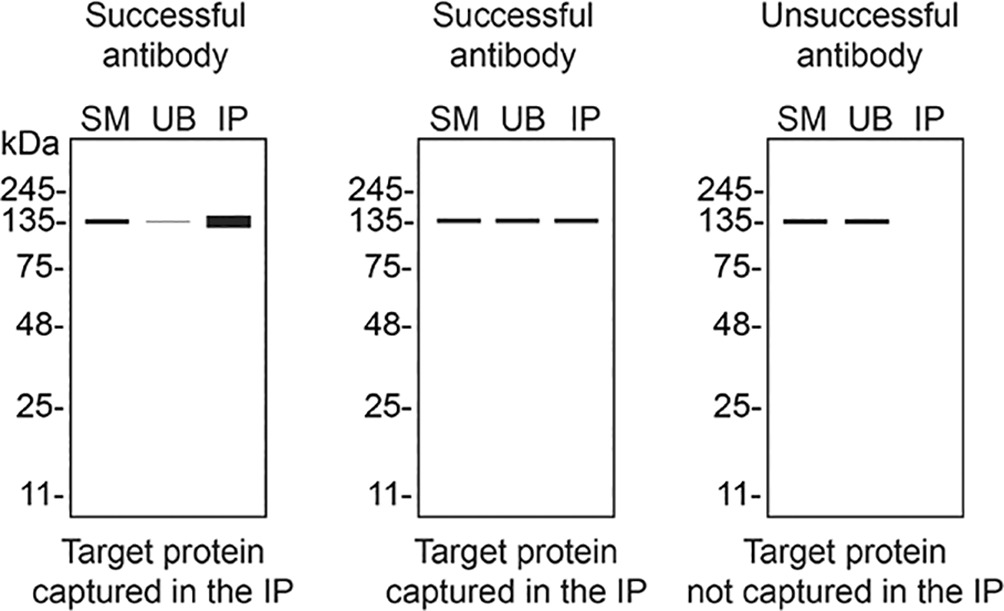
\includegraphics[width=0.9\textwidth]{img/antibody_val/ycharos_ip.jpg}
    \caption*{Schematic illustrating expected outcomes for a successful antibody that heavily depletes the target protein from the SM (left), a successful antibody that less heavily depletes the target protein from the SM (center) and a non-successful antibody (right). Adapted from Table 3 of \href{https://doi.org/10.12688/f1000research.155929.2}{Ru\'iz Mole\'on et al. (2025)}.}
\end{figure}

\pagebreak

\subsection*{Immunofluorescence}

In immunofluorescence, cells are \href{https://en.wikipedia.org/wiki/Fixation_(histology)}{fixed}, \href{https://doi.org/10.1007/978-1-59745-324-0_9}{permeabilized} and stained with an antibody conjugated to a fluorophore. This antibody will bind to the protein of interest within the cell, localize itself to the region of the cell that the protein inhabits. To validate antibodies with immunofluorescence, YCharOS takes fluorescence images of WT and KO cells plated together as a `mosaic'.  The WT and KO cells are labeled with fluorophores of different wavelengths so that they can be differentiated from one another. For intracellular proteins (i.e., not secreted), fluorescence signal for the protein of interest should be pronounced in the WT cell line, negligible in the KO cell line and negligible in the background. 

Antibodies that are successful for immunofluorescence generally target the protein of interest in its native, folded state. YCharos \href{https://f1000research.com/gateways/ycharos/faqs}{states}:

\begin{quote}
    \textit{A successful antibody immunolocalizes the target protein by generating a signal in WT cells that is at least 1.5-fold over the signal in KO cells. Signal provided by such antibody can be easily distinguished from background noise.}
\end{quote}

\begin{figure}[h!tbp]
    \centering
    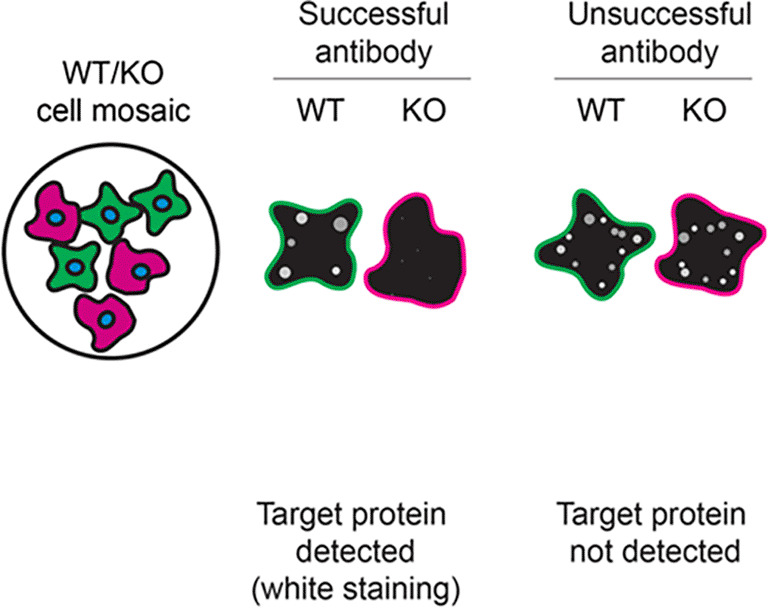
\includegraphics[width=0.9\textwidth]{img/antibody_val/ycharos_if.jpg}
    \caption*{Schematic illustrating expected outcomes for a successful antibody that localizes to the protein of interest in the WT but not KO (left) and an unsuccessful antibody that does not localize to the protein of interest (as made evident by the equivalent signal in the KO cell line, right).}
\end{figure}

\subsection*{Example 1: Bax Antibody (B-9)}

Bax Antibody (B-9) (sold by Santa Cruz Biotechnology under catalog number \href{https://www.scbt.com/p/bax-antibody-b-9}{sc-7480}) has been used in more than 1,000 articles to target \href{https://en.wikipedia.org/wiki/Apoptosis_regulator_BAX}{Bax}, a widely-studied regular of apoptosis, in rat, mouse and human cells. However, \href{https://doi.org/10.1038/s41419-024-07273-6}{Entrop et al. (2024)} report on validation studies using using WT and Bax-deficient cell lines (as well as cell lines through which Bax has been depleted with \href{https://en.wikipedia.org/wiki/Small_interfering_RNA}{siRNA}) through which they find that Bax Antibody (B-9) likely does not target Bax. Instead, the antibody likely targets another protein at a similar molecular weight. Bax is a widely-studied gene and there are hundreds of other Bax-targeting antibodies available from a number of providers.

\subsection*{Additional resources}

\begin{itemize}
    \setlength\itemsep{-0.5em}
    \item \href{https://doi.org/10.1038/s41596-024-01108-6}{``YCharOS protocol for antibody validation'' (2024)}
    \item \href{https://f1000research.com/ycharos}{YCharOS F1000 Research Gateway}
    \item \href{https://zenodo.org/communities/ycharos/records?q=&l=list&p=1&s=10&sort=newest}{YCharos Zenodo community}
    \item \href{https://doi.org/10.1038/d41586-024-03590-0}{``The antibodies don’t work! The race to rid labs of molecules that ruin experiments'' (2024)}
    \item \href{https://doi.org/10.1038/521274a}{``Reproducibility crisis: Blame it on the antibodies'' (2015)}
    \item \href{https://doi.org/10.1038/nmeth.3472}{``Assessment of a method to characterize antibody selectivity and specificity for use in immunoprecipitation'' (2015)}
    \item \href{https://doi.org/10.1038/s41419-024-07273-6}{``Why Bax detection in >1400 publications might be flawed'' (2024)}
    \item \href{https://doi.org/10.1007/s00210-009-0395-y}{``How reliable are G-protein-coupled receptor antibodies?'' (2009)}
\end{itemize}

\end{document}